\chapter{Математические модели}
Решение рассматриваемой задачи, основанное на степенной связи интенсивности напряжений и скоростей деформации ползучести при напряжениях, не превосходящих предела текучести материала, представлено в монографии Л.М.Качанова [\ref{kachanov}].
Решение задачи о деформировании мембраны в стесненных условиях при учете упрочнения материала приведены в монографиях Н.Н.~Малинина, [\ref{malinin}] и К.И. Романова [\ref{romanov}]. Известные работы [\ref{malinin},\ref{jerebcov}] допускают появление нефизичных бесконечных напряжений ($\sigma_u \to \infty$) в начальный момент времени, для их исключения в данной работе дополнительно учитывается мгновенное деформирование.
В [\ref{teraud_dis}, \ref{teraud}] приведено решение рассматриваемой задачи при различных граничных условиях, однако только для клиновидной матрицы. В данной работе приводится обобщение результатов, полученных в [\ref{teraud_dis}, \ref{teraud}], на случай криволинейной матрицы. Напряженное состояние мембраны можно считать безмоментным. Поскольку длина мембраны значительно превосходит её ширину, можно считать, что реализуется случай плоской деформации.

\section{Деформирование внутри криволинейной матрицы \label{section_1_1}}
	\begin{figure}[h!]
		\begin{minipage}[h]{0.48\linewidth}
			\center{\includegraphics[width=1.0\linewidth]{images/creep.eps}}
			\caption{ \textbf{НЕПРАВИЛЬНАЯ} Криволинейная матрица} 
		\end{minipage}
		\hfill
		\begin{minipage}[h]{0.48\linewidth}
Первая стадия~--- стадия мгновенного упругого деформирования позволяет моделировать процесс деформации в начальный момент времени, для исключения есконечных
	напряжений при $t ~ 0$
	Упругое деформирование мембраны описывается помощью закона Гука при сложном напряженном состоянии при учете несжимаемости материала мембраны.
		\end{minipage}
		\label{quad_matrix}
	\end{figure}
	\subsection{Первая стадия}
	
	
	Вводим безразмерные переменные:
	\begin{equation}
		\overline{q} = \dfrac{q}{\sigma_b}, \;
		\overline{H} = \dfrac{H}{H_0}, \;
		\overline{H}_0 = \dfrac{H_0}{a}, \;
		\overline{t} = \dfrac{\sqrt 3}{2}Ct,\;
		k = \dfrac{E}{\sigma_b},\;
		\overline{\rho} = \dfrac{\rho}{H_0},
	\end{equation}
	где где $H$ ~--- толщина мембраны в произвольный момент времени, $H_0$~--- толщина мембраны при $t = -0$, $q$~--- давление, $2a$~--- ширина,
	$E$~--- модуль Юнга, $\rho$ толщина и радиус кривизны мембраны.
	При дальнейшем анализе черточки над безразмерными величинамиd этом пункте  опустим. Так как вывод формул описан в работах  [\ref{teraud_dis}, \ref{teraud}]
	и совпадает с нашим решением, приведем только итоговый результат, описывающий связь давления $q$ и мгновенно появляющегося угла $\alpha_1$,
	также приведены характеристики, описывающие состояние мембраны($H_1$~--- толщины и $\sigma_{\theta1}$):

	\begin{equation}
	\begin{split}
		q = \dfrac43 H_0k\sin(\alpha_1)\left(1-\dfrac{\sin(\alpha_1)}{\alpha_1} \right), \\
		H_1 = \dfrac{\sin(\alpha_1)}{\alpha_1},\\
		\sigma_{\theta1} = \dfrac{q}{H_1H_0\sin(\alpha_1)},
	\end{split}
	\label{guk_deformation}
	\end{equation}
	
	Следует отметить, что соотношения (\ref{guk_deformation}) позволяют исключить бесконечные напряжения в начальный момент времени.
	Так же следует отметить, что в работе расчет этих значений для материала были произведены с помощью программного средства Maxima.
	 
	\subsection{Вторая стадия}
	Вторая стадия~--- стадия свободного деформирования позволяет моделировать 
	деформацию мембраны вплоть до её касания стенок матрицы, что соответствует углу раствора $2\alpha_2$. Подробное описание вывода соотношений описано в работах  [\ref{teraud_dis}, \ref{teraud}], поэтому приведем то соотношение, которое было рассмотрено и реализовано в работе:
	\begin{equation}
	\label{free_deformation}
	\end{equation}
	
	Для анимированного моделирования деформации мембраны требовались промежуточные
	расчетов по формуле (\ref{free_deformation}), которые были произведены методами: 
	\ref{gauss}, \ref{simpson}
	\subsection{Третья стадия}
ПОСМОТРИ КАК В СТАТЬЕ
	Началом стесненного деформирования (третья стадия) считается момент времени, при котором мембрана впервые касается матрицы. При исследовании этой стадии рассматривается идеальное скольжение мембраны вдоль матрицы, поверхность которой задана уравнением $y = f(x) = b(1-x^k)$ c соответствующими ограничениями $x\in [-1,1], \; y \in [0, b]$. При этом на матрицу будет наложено ограничение, аналогичное 
[ref{jerebcov}]: кривизна кривой должна монотонно увеличиваться от точки $a$ до $0$, для того, чтобы зона стесненного деформирования оставалась одна.

Рассмотрим аналогично [\ref{jerebcov}] два близких деформированных состояния:
одно  с радиусом $\rho$ и длиной участка контакта $s$ и второе $\rho+d\rho$ и длиной участка контакта $s+ds$. Основываясь на геометрических соображениях (\ref{quad_matrix}), получим соотношения, характеризующие два близких состояния в данных координатных осях:
\begin{eqnarray}
\left. 
\begin{split}
\rho(x_0) &= \sqrt{(y_0-y_c)^2 + x_0^2};\; d\rho = \rho'_{x_0}dx_0\\
s(x_0) &= \int\limits^1_{x_0}\sqrt{1+f_x'^2}\,dx; \; ds = s'_{x_0}dx_0\\
\alpha(x_0)&= \dfrac{\pi}{2} - \arctg(g'_{x_0});\; d\alpha = \alpha'_{x_0}dx_0
\end{split}
\right\}
\end{eqnarray}

где $H$ ~--- толщина мембраны, $q$~--- давление, $H_0$~--- начальная толщина, $C$~---  константа материала, $a$~--- ширина,    Где $x_0$~--- крайняя точка касания мембраны стенок матрицы, $\rho=\rho(x_0), \alpha=\alpha(x_0)$~--- радиус кривизны и угол раствора свободной части мембраны, $s=s(x_0)$~--- длина участка контакта,
$g(x_0)$~-- нормаль к функции профиля матрицы. 
Учитывая идеальное скольжение мембраны вдоль стенок матрицы, её геометрических характеристиках, получим соотношение для окружной деформации ползучести:

\begin{equation}
p_\theta = \dfrac{\rho d\alpha +\alpha d\rho+ds}{\rho\alpha+s}
\label{deformation_quad_matrix}
\end{equation}
Каждое из слагаемых числителя (\ref{deformation_quad_matrix}) содержит $dx_0$, то можно сгруппировать и ввести обозначения: 
\begin{equation}
\rho d\alpha + \alpha d\rho +ds = B_1(x_0)dx_0;\; \rho\alpha+s = B_2(x_0).
\end{equation}

Тогда 
\begin{equation}
	dp_\theta = \dfrac{B_1(x_0)dx_0}{B_2(x_0)}
	\label{deformation_quad_matrix_ideal}
\end{equation}
 
 С помощью (\ref{deformation_quad_matrix_ideal}) вычисляем характеристики деформированного состояния:
 \begin{equation}
 \dot{p_\theta} = \dfrac{B_1}{B_2}\dfrac{dx_0}{dt};\;
 \dot{p_u}  = \dfrac{2}{\sqrt3} \dfrac{B_1}{B_2}\dfrac{dx_0}{dt}
 \end{equation}
 
 Аналогично выводам [\ref{jerebcob}], из условия несжимаемости плоского деформированного состояния получаем:
 \begin{equation}
 H=H_1\exp\left(\int\limits_1^{x_0}\dfrac{B_1}{B_2}dx_0\right)
  \label{quad_matrix_h}
 \end{equation}
 
 Интенсивность напряжений будет:
 \begin{equation}
 \sigma_u = \dfrac{\sqrt 3}{2}\sigma_\theta = \dfrac{\sqrt 3}{2}\dfrac{q\rho}{H}
 \label{sigma}
 \end{equation}
 
 Подставляя (\ref{deformation_quad_matrix_ideal}), (\ref{sigma})в (\ref{main_equation}) получим выражение, характеризующее зависимость $x_0(t)$:
 
 \begin{equation}
   t = t_1 + \int\limits^{x_0}_1 \left[ \dfrac{2H}{\sqrt3 q \rho} -1\right]^n\dfrac{B_1}{B_2}\,dx_0,
   \end{equation}
где $t_1$~-- время окончания стадии свободного деформирования.   
Выражение подлежит численному исследованию, результаты которого приведены \ref{chapter_2}

\section{Деформирование внутри матрицы с вертикальными стенками и плоским днищем}
	\subsection{Первая и вторая стадия}
		Первая ти вторая стадия не имеют отличительных особенностей по сравнению 
		с моделированием деформирования внутри криволинейной матрицы. Поэтому 
		при вычислениях были взяты формулы (\ref{guk_deformation}) и (\ref{free_deformation}).
	\subsection{Третья и четвертая стадия}
	При рассмотрении матрицы с вертикальными стенками и плоским днищем учитывалось, 
	что стесненное деформирование проходит как две последовательные стадии: 
	третья стадия~--- когда мембрана касается только стенок матрицы и четвертая 
	стадия~--- когда мембрана касается днища матрицы и свободных дуг становится две.
	
	
	Дана матрица шириной $2a$ и высотой $L$.
	Рассмотрим два близких состояния в третьей стадии:
	одно  с радиусом $\rho$ и длиной участка контакта $s$ и с длиной участка контакта $s+ds$. При касании только вертикальных стенок радиус свободной дуги матрицы изменятся не будет, поэтому: 
\begin{equation}
dp = \dfrac{ds}{s+\frac{pi}{2}\rho}
\label{vertikal_matrix_trird}
\end{equation}

Введем безразмерные величины:
\begin{equation}
\overline{\rho} = \dfrac{\rho}{\alpha}, \overline{s}=\dfrac{s}{a},
\label{parall_variables_no_dimention}
\end{equation}

Подставляя (\ref{parall_variables_no_dimention}) в (\ref{vertikal_matrix_trird}) и учитывая, что из геометрического смысла на этом этапе $\rho = a$, получим(черточки над безразмерными переменными опустим):
	\begin{equation}
	dp = \dfrac{ds}{s+\frac{\pi}{2}}
	\label{vertikal_matrix_trird_nodim}
	\end{equation}

Перейдем к координатам, аналогично пункту \ref{section_1_1}, введя тривиальную зависимость точки прилипания от координаты касания: $s=y, ds = dy$.
Проведя замену переменных и учитывая условие несжимаемости плоского деформированного состояния получаем:
	\begin{equation}
	H=\dfrac{H_1(y+\frac{pi}{2})}{\frac{\pi}{2}}
	\end{equation}
Поставляя (\ref{vertikal_matrix_trird_nodim}), (\ref{sigma}) в (\ref{main_equation}) и используя замену переменных получим:
\begin{equation}
t = t_1 + \int\limits_0^{y_0}\left[ \dfrac{2H}{\sqrt3 q \rho} -1\right]^n\left(\dfrac{dy_0}{y_0+\frac{\pi}{2}}\right)
\end{equation}
	где $t_1$~-- время окончания стадии свободного деформирования.   
Выражение подлежит численному исследованию, результаты которого приведены \ref{chapter_2}

	

	
	Рассмотрим два близких состояния при касании мембраны днища матрицы:
	одно  с радиусом $\rho$ и длиной участка контакта $s$ и другое с радиусом $\rho$с длиной участка контакта $s+ds$.
	\begin{equation}
	% это формула для 4 стадии
	p_\theta = \dfrac{2ds+\frac{\pi}{2}d\rho}{L-a+2s+\frac{\pi}{2}},
	\end{equation}

